%*******************************************************************************
%*********************************** Fifth Chapter *****************************
%*******************************************************************************

\chapter{Density Measurement Induced Dynamics}
% Title of the Fifth Chapter

\ifpdf
    \graphicspath{{Chapter5/Figs/Raster/}{Chapter5/Figs/PDF/}{Chapter5/Figs/}}
\else
    \graphicspath{{Chapter5/Figs/Vector/}{Chapter5/Figs/}}
\fi


\section{Introduction}

In the previous chapter we have introduced a theoretical framework
which will allow us to study measurement backaction using
discontinuous quantum jumps and non-Hermitian evolution due to null
outcomes. We have also wrapped our quantum gas model in this quantum
trajectory formalism by considering ultracold bosons in an optical
lattice coupled to a cavity which collects and enhances light
scattered in one particular direction. One of the most important
conclusions of the previous chapter was that the introduction of
measurement introduces a new energy and time scale into the picture.

In this chapter, we investigate the effect of quantum measurement
backaction on the many-body state of atoms. In particular, we will
focus on the competition between the backaction and the the two
standard short-range processes, tunnelling and on-site interactions,
in optical lattices. We show that the possibility to spatially
structure the measurement at a micrscopic scalecomparable to the
lattice period without the need for single site resolution enebales us
to engineer efficient competition between the three processes in order
to generate new nontrivial dynamics. Furthermore, the global nature of
the measurement creates long-range correlations which enable nonlocal
dynamical processes distinguishing it from the local processes.

In the weak measurement limit, where the quantum jumps do not occur
frequently compared to the tunnelling rate, this can lead to global
macroscopic oscillations of bosons between odd and even sites. These
oscillations occur coherently across the whole lattice enabled by the
fact that measurement is capable of generating nonlocal spatial modes.

When on-site interactions are included in the picture we obtain a
system with three competing energy scales of which two correspond to
local processes and one is global. This complicates the picture
immensely. We show how under certain circumstances interactions
prevent measurement from generating globally coherent dynamics, but on
the other hand when the measurement is strong both processes
collaborate in squeezing the atomic distribution.

On the other end of the spectrum, when measurement is strong we enter
the regime of quantum Zeno dynamics. Frequent measurements can slow
the evolution of a quantum system leading to the quantum Zeno effect
where a quantum state is frozen in its initial configuration. One can
also devise measurements with multi-dimensional projections which lead
to quantum Zeno dynamics where unitary evolution is uninhibited within
this degenrate subspace, i.e.~the Zeno subspace. The flexible setup
where global light scattering can be engineered allows us to suppress
or enhance specific dynamical processes thus realising spatially
nonlocal quantum Zeno dynamics. This unconventional variation of
quantum Zeno dynamics occurs when measurement is near, but not in, its
projective limit. The system is still confined to Zeno subspaces, but
intermediate transitions are allowed via virtual Raman-like
processes. We show that this result can, in general (i.e.~beyond the
ultracold gas model considered here), be approimated by a
non-Hermitian Hamiltonian thus extending the notion of quantum Zeno
dynamics into the realm of non-Hermitian quantum mechanics joining the
two paradigms.

The measurement process generates spatial modes of matter fields that
can be considered as designed systems and reservoirs opening the
possibility of controlling dissipations in ultracold atomic systems
without resorting to atom losses and collisions which are difficult to
manipulate. The continuous measurement of the light field introduces a
controllable decoherence channel into the many-body
dynamics. Furthermore, global light scattering from multiple lattice
sites creates nontrivial spatially nonlocal coupling to the
environment which is impossible to obtain with local
interactions. Such a quantum optical approach can broaden the field
even further allowing quantum simulation models unobtainable using
classical light and the design of novel systems beyond condensed
matter analogues.

\section{Large-Scale Dynamics due to Weak Measurement}

We start by considering the weak measurement limit when photon
scattering does not occur frequently compared to the tunnelling rate
of the atoms, i.e.~$\gamma \ll J$. When the system is probed in this
way, the measurement is unable to project the quantum state of the
bosons to an eigenspace thus making it impossible to establish quantum
Zeno Dynamics. However, instead of confining the evolution of the
quantum state, it has been shown in Refs. \cite{mazzucchi2016,
  mazzucchi2016njp} that the measurement leads to coherent global
oscillations between the modes generated by the spatial profile of the
light field. Fig. \ref{fig:oscillations} illustrates the atom number
distributions in one of the modes for $Z = 2$ ($N_\mathrm{odd}$) and
$Z = 3$ ($N_1$) \cite{mazzucchi2016}. In the absence of the external
influence of measurement these distributions would spread out
significantly and oscillate with an amplitude that is less than or
equal to the initial imbalance, i.e.~small oscillations for a small
initial imbalance. By contrast, here we observe a macroscopic exchange
of atoms between the modes even in the absence of an initial
imbalance, that the distributions consist of a small number of well
defined components, and these components are squeezed by the weak
measurement.

\begin{figure}[htbp!]
  \centering
  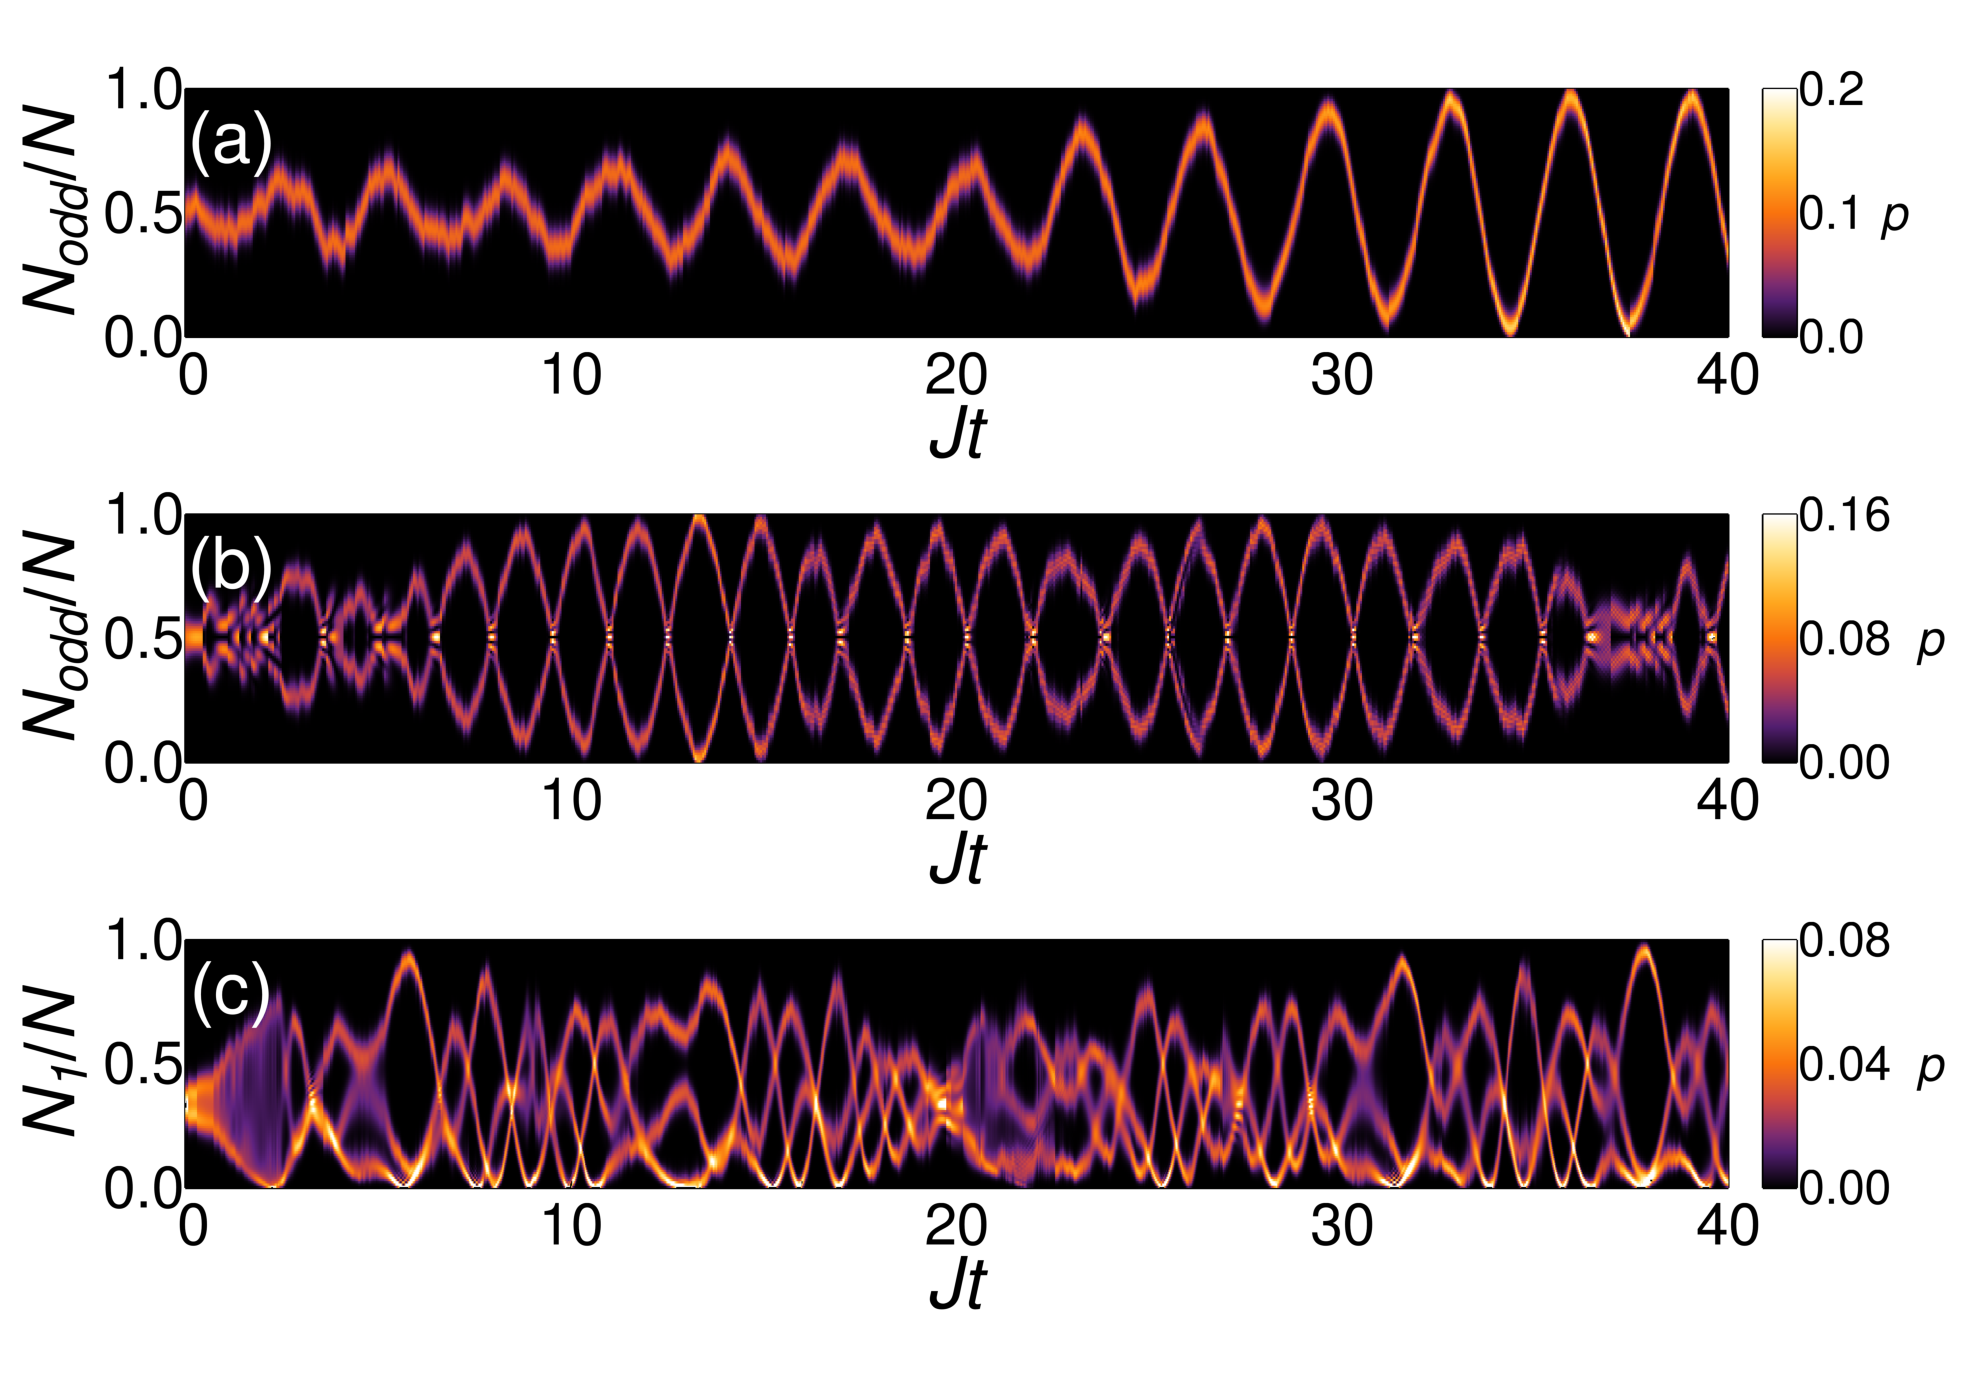
\includegraphics[width=\textwidth]{Oscillations}
  \caption[Macroscopic Oscillations due to Weak Measurement]{Large
    oscillations between the measurement-induced spatial modes
    resulting from the competition between tunnelling and weak
    measurement induced backaction. The plots show the atom number
    distributions $p(N_l)$ in one of the modes in individual quantum
    trajectories. These dstributions show various numbers of
    well-squeezed components reflecting the creation of macroscopic
    superposition states depending on the measurement
    configuration. $U/J = 0$, $\gamma/J = 0.01$, $M=N$, initial
    states: bosonic superfluid. (a) Measurement of the atom number at
    odd sites $\hat{N}_\mathrm{odd}$ creates one strongly oscillating
    component in $p(N_\mathrm{odd})$ ($N = 100$ bosons, $J_{j,j} = 1$
    if $j$ is odd and 0 otherwise). (b) Measurement of
    $(\hat{N}_\mathrm{odd} - \hat{N}_\mathrm{even})^2$ introduces
    $Z = 2$ modes and preserves the superposition of positive and
    negative atom number differences in $p(N_\mathrm{odd})$ ($N = 100$
    bosons, $J_{j,j} = (-1)^{j+1}$). (c) Measurement for $Z = 3$ modes
    preserves three components in $p(N_1)$ ($N = 108$ bosons,
    $J_{j,j} = e^{i 2 \pi j / 3}$.}
  \label{fig:oscillations}
\end{figure}

Furthermore, depending on the quantity being addressed by the
measurement, the state of the system has multiple components as seen
in Figs. \ref{fig:oscillations}b and \ref{fig:oscillations}c. This is a
consequence of the fact that the measured light intensity $\ad_1 \a_1$
is not sensitive to the light phase. The measurement will not
distinguish between all permutations of mode occupations that scatter
light with the same intensity, but different phase. For example, when
measuring $\hat{D} = \hat{N}_\mathrm{odd} - \hat{N}_\mathrm{even}$,
the light intensity will be proportional to
$\hat{D}^\dagger \hat{D} = (\hat{N}_\mathrm{odd} -
\hat{N}_\mathrm{even})^2$ and thus it cannot distinguish between a
positive and negative imbalance leading to the two components seen in
Fig. \ref{fig:oscillations}. More generally, the number of components
of the atomic state, i.e.~the degeneracy of $\ad_1 \a_1$, can be
computed from the eigenvalues of Eq. \eqref{eq:Zmodes}, 
\begin{equation}
  \hat{D} = \sum_l^Z \exp\left[-i 2 \pi l R / Z \right] \hat{N}_l,
\end{equation}
noting that they can be represented as the sum of vectors on the
complex plane with phases that are integer multiples of $2 \pi / Z$:
$N_1 e^{-i 2 \pi R / Z}$, $N_2 e^{-i 4 \pi R / Z}$, ..., $N_Z$. Since
the set of possible sums of these vectors is invariant under rotations
by $2 \pi l R / Z$, $l \in \mathbb{Z}$, and reflection in the real axis, the
state of the system is 2-fold degenerate for $Z = 2$ and $2Z$-fold
degenerate for $Z > 2$. Fig. \ref{fig:oscillations} shows the three
mode case, where there are in fact $6$ components ($2Z = 6$), but in
this case they all occur in pairs resulting in three visible
components.

It has also been shown in Ref. \cite{mazzucchi2016njp} that the
non-interacting dynamics with quantum measurement backaction for
$R$-modes reduce to an effective Bose-Hubbard Hamiltonian with
$R$-sites provided the initial state is a superfluid. In this
simplified model the $N_j$ atoms in the $j$th site corresponds to a
superfluid of $N_j$ atoms within a single spatial mode as defined by
Eq. \eqref{eq:Zmodes}. Furthermore, the tunnelling term in the
Bose-Hubbard model and the quantum jumps do not affect this
correspondence.

Therefore, we will now consider an illumination pattern with
$\hat{D} = \hat{N}_\mathrm{odd}$. This pattern can be obtained by
crossing two beams such that their projections on the lattice are
identical and the even sites are positioned at their
nodes. Fig. \ref{fig:oscillations}a shows that this leads to
macroscopic oscillations with a single peak. We will now attempt to
get some physical insight into the process by using the reduced
effective double-well model. The atomic state can be written as 
\begin{equation}
  \label{eq:discretepsi}
  | \psi \rangle = \sum_l^N q_l |l, N - l \rangle,
\end{equation}
where the ket $| l, N - l \rangle$, represents a superfluid with $l$
atoms in the odd sites and $N-l$ atoms in the even sites. The
non-Hermitian Hamiltonian describing the time evolution in between the
jumps is given by
\begin{equation}
  \label{eq:doublewell}
  \hat{H} = -J^\mathrm{cl} \left( \bd_o b_e + b_o \bd_e \right) - i
  \gamma \n_o^2
\end{equation}
and the quantum jump operator which is applied at each photodetection
is $\c = \sqrt{2 \kappa} C \n_o$. $b_o$ ($\bd_o$) is the
annihilation (creation) operator in the left-hand site in the
effective double-well corresponding to the superfluid at odd sites of
the physical lattice. $b_e$ ($\bd_e$) is defined similarly, but for
the right-hand site and the superfluid at even sites of the physical
lattice. $\n_o = \bd_o b_o$ is the atom number operator in the
left-hand site.

Even though Eq. \eqref{eq:doublewell} is relatively simple as it it is
only a non-interacting two-site model, the non-Hermitian term
complicates the situation making the system difficult to
solve. However, a semiclassical approach to boson dynamics in a
double-well in the limit of many atoms $N \gg 1$ has been developed in
Ref. \cite{juliadiaz2012}. It was originally formulated to treat
squeezing in a weakly interacting bosonic gas, but it can be easily
applied to our system as well. In the limit of large atom number, the
wavefunction in Eq. \eqref{eq:discretepsi} can be described using
continuous variables by defining $\psi (x = l / N) = \sqrt{N}
q_l$. Note that this requires the coefficients $q_l$ to vary smoothly
which is the case for a superfluid state. We now rescale the
Hamiltonian in Eq. \eqref{eq:doublewell} to be dimensionless by
dividing by $NJ$ and define the relative population imbalance between
the two wells $z = 2x - 1$. Finally, by taking the expectation value
of the Hamiltonian and looking for the stationary points of
$\langle \psi | \hat{H} | \psi \rangle - E \langle \psi | \psi
\rangle$ we obtain the semiclassical Schr\"{o}dinger equation
\begin{equation}
  \label{eq:semicl}
  i h \partial_t \psi(z, t) = \mathcal{H} \psi(z, t),
\end{equation}
\begin{equation}
  \label{eq:semiH}
  \mathcal{H} \approx -2 h^2 \partial^2_z \psi(z, t) + \left[
    \frac{\omega^2 z^2} {8} - \frac{i \Gamma} {4} \left( z + 1
    \right)^2 \right] \psi(z, t),
\end{equation}
where $\Gamma = N \kappa |C|^2 / J$, $h = 1/N$,
$\omega = 2 \sqrt{1 + \Lambda - h}$, and
$\Lambda = NU / (2J^\mathrm{cl})$. We will be considering $U = 0$ as
the effective model is only valid in this limit, thus $\Lambda =
0$. However, this model is valid for an actual physical double-well
setup in which case interacting bosons can also be considered. The
equation is defined on the interval $z \in [-1, 1]$, but we have
assumed that $z \ll 1$ in order to simplify the kinetic term and
approximate the potential as parabolic. This does mean that this
approximation is not valid for the maximum amplitude oscillations seen
in Fig. \ref{fig:oscillations}a, but since they already appear early
on in the trajectory we are able to obtain a valid analytic
description of the oscillations and their growth.

A superfluid state in our continuous variable approximation
corresponds to a Gaussian wavefunction $\psi$. Furthermore, since the
potential is parabolic even with the inclusion of the non-Hermitian
term, it will remain Gaussian during subsequent time
evolution. Therefore, we will use a very general Gaussian wavefunction
of the form
\begin{equation}
  \label{eq:ansatz}
  \psi(z, t) = \frac{1}{\pi b^2}\exp\left[ i \epsilon 
  - \frac{(z - z_0)^2} {2 b^2} + \frac{i \phi (z - z_\phi)^2} {2 b^2} \right]
\end{equation}
as our ansatz to Eq. \eqref{eq:semicl}. The parameters $b$, $\phi$,
$z_0$, and $z_\phi$ are real-valued functions of time whereas
$\epsilon$ is a complex-valued function of time. Physically, the value
$b^2$ denotes the width, $z_0$ the position of the center, and $\phi$
and $z_\phi$ contain the phase information of the Gaussian wave
packet.

The non-Hermitian Hamiltonian and an ansatz are not enough to describe
the full dynamics due to measurement. We also need to derive the
effect of a single quantum jump. Within the continuous variable
approximation, our quantum jump become $\c \propto 1 + z$. We neglect
the constant prefactors, because the wavefunction is normalised after
a quantum jump. Expanding around the peak of the Gaussian ansatz we
get
\begin{equation}
  1 + z \approx \exp \left[ \ln (1 + z_0) + \frac{z - z_0}{1 + z_0} -
    \frac{(z - z_0)^2}{2 (1 + z_0)^2} \right].
\end{equation}
Multiplying the wavefunction in Eq. \eqref{eq:ansatz} with the jump
operator above yields a Gaussian wavefunction as well, but the
parameters change discontinuously according to
\begin{align}
  \label{eq:jumpb2}
  b^2 & \rightarrow \frac{ b^2 (1 + z_0)^2 } { (1 + z_0)^2 + b^2 }, \\
  \phi & \rightarrow \frac{ \phi (1 + z_0)^2 } { (1 + z_0)^2 + b^2 }, \\
  \label{eq:jumpz0}
  z_0 & \rightarrow z_0 + \frac{ b^2 (1 + z_0) } { (1 + z_0)^2 + b^2}, \\
  z_\phi & \rightarrow z_\phi.
\end{align}
The fact that the wavefunction remains Gaussian after a photodetection
is a huge advantage, because it means that the combined time evolution
of the system can be described with a single Gaussian ansatz in
Eq. \eqref{eq:ansatz} subject to non-Hermitian time evolution
according to Eq. \eqref{eq:semicl} with discontinous changes to the
parameter values at each quantum jump.

Having identified an appropriate ansatz and the effect of quantum
jumps we proceed with solving the dynamics of wavefunction in between
the photodetecions. The initial values of the parameters for a
superfluid state of $N$ atoms across the whole lattice are $b^2 = 2h$,
$\phi =0$, $a_0 = 0$, and $a_\phi = 0$. Howver, we use the most
general initial conditions at time $t = t_0$ which we denote by
$b(t_0) = b_0$, $\phi(t_0) = \phi_0$, $z_0(t_0) = a_0$, and
$z_\phi(t_0) = a_\phi$. The reason for keeping them as general as
possible is that after every quantum jump the system changes
discontinuously. The subsequent time evolution is obtained by solving
the Schr\"{o}dinger equation with the post-jump paramater values as
the new initial conditions.

By plugging the ansatz in Eq. \eqref{eq:ansatz} into the
Eq. \eqref{eq:semicl} we obtain three differential equations
\begin{equation}
  \label{eq:p}
  -2 h^2 p^2 + \left( \frac{ \omega^2 } { 8 } - \frac{ i \Gamma } { 4
    } \right) + \frac{ i h } { 2 } \frac{ \mathrm{d} p } { \mathrm{d}
    t } = 0,
\end{equation}
\begin{equation}
  \label{eq:pq}
  4 h^2 p q - \frac{ i \Gamma } { 2 } - i h \frac{ \mathrm{d} q } {
    \mathrm{d} t } = 0
\end{equation}
\begin{equation}
  \label{eq:pqr}
  -2 h^2 (q^2 - p) - \frac{ i \Gamma } { 4 } - i h \left( \frac{ 1 } {
      4 x } \frac{ \mathrm{d} x } {\mathrm{d} t } + i \frac{
      \mathrm{d} \epsilon } { \mathrm{d} t } - \frac{1}{2} \frac{
      \mathrm{d} r } { \mathrm{d} t } \right) = 0,
\end{equation}
where $x = 1/b^2$, $p = (1 - i \phi)/b^2$,
$q = (z_0 - i \phi z_\phi)/b^2$, and
$r = (z_0^2 - \phi z_\phi^2)/b^2$. The corresponding initial
conditions are $x(0) = x_0 = 1/b_0^2$,
$p(0) = p_0 = (1 - i \phi_0)/b_0^2$,
$q(0) = q_0 = (a_0 - \phi_0 a_\phi)/b_0^2$, and
$r(0) = r_0 = (a_0^2 - \phi_0 a_\phi^2)/b_0^2$. The original
parameters can be extracted from these auxiliary variables by
$b^2 = 1 / \Re \{ p \}$, $\phi = - \Im \{ p \} / \Re \{ p \}$,
$z_0 = \Re \{ q \} / \Re \{ p \}$,
$z_\phi = \Im \{ q \} / \Im \{ p \}$, and $\epsilon$ is appears
explicitly in the equations above.

First, it is worth noting that all parameters of interest can be
extracted from $p(t)$ and $q(t)$ alone. We are not interested in
$\epsilon$ as it is only related to the global phase and the norm of
the wavefunction and it contains little physical
information. Furthermore, an interesting and incredibly convenient
feature of these equations is that the Eq. \eqref{eq:p} is a function
of $p(t)$ alone and Eq. \eqref{eq:pq} is a function of $p(t)$ and
$q(t)$ only. Therefore, we only need to solve first two equations and
we can neglect Eq. \eqref{eq:pqr}.

Eq. \eqref{eq:p} can be rearranged into the form
\begin{equation}
  \frac{ \mathrm{d} p } { (\zeta \omega / 4 h)^2 - p^2 } = i 4 h
  \mathrm{d} t,
\end{equation}
where $\zeta^2 = (\alpha - i \beta)^2 = 1 - i 2 \Gamma / \omega^2$, and
\begin{equation}
  \alpha = \sqrt{ \frac{1}{2} + \frac{1}{2} \sqrt{1 + \frac{ 4\Gamma^2
      }{ \omega^4 }}},
\end{equation}
\begin{equation}
  \beta = -\sqrt{ -\frac{1}{2} + \frac{1}{2} \sqrt{1 + \frac{ 4\Gamma^2
      }{ \omega^4 }}}.
\end{equation}
This is a standard integral\footnotemark and thus yields
\begin{equation}
  \label{eq:psol}
  p(t) = \frac{ \zeta \omega } { 4 h } 
  \frac{ ( \zeta \omega + 4 h p_0 )e^{i \zeta \omega t} - ( \zeta
    \omega - 4 h p_0 ) e^{-i \zeta \omega t} }
  { ( \zeta \omega + 4 h p_0 )e^{i \zeta \omega t} + ( \zeta \omega
    - 4 h p_0 ) e^{-i \zeta \omega t} }.
\end{equation}

\footnotetext{ \[ \int \frac{\mathrm{d} x}{a^2 - x^2} = \frac{1}{2a}
    \ln \left( \frac{a+x}{a-x} \right) + \mathrm{const.} 
    \quad\quad\quad\quad\quad\quad\quad\quad\quad\quad\quad\quad\quad\quad\quad
    \quad\quad\quad\quad\quad\] }

Having found an expression for $p(t)$ we can now solve
Eq. \eqref{eq:pq} for $q(t)$. To do that we first define the
integrating factor
\begin{equation}
  I(t) = \exp \left[ i 4 h \int p \mathrm{d} t \right],
\end{equation}
which lets us rewrite Eq. \eqref{eq:pq} as
\begin{equation}
  \frac{\mathrm{d}} {\mathrm{d} t}(Iq) = - \frac{\Gamma}{2 h} I.
\end{equation}
Upon integrating the equation above we obtain
\begin{equation}
  \label{eq:Iq}
  Iq = - \frac{ \Gamma } {2 h} \int I \mathrm{d} t.
\end{equation}
The integrating factor can be evaluated and shown to be
\begin{equation}
  I(t) = ( \zeta \omega + 4 h p_0 )e^{i \zeta \omega t} + 
  ( \zeta \omega - 4 h p_0 )e^{-i \zeta \omega t},
\end{equation}
which upon substitution into Eq. \eqref{eq:Iq} yields the solution
\begin{equation}
  \label{eq:qsol}
  q(t) = \frac{1}{2 h \zeta \omega} 
  \frac{4 h \zeta^2 \omega^2 q_0 - i 8 h \Gamma p_0
    + i \Gamma [( \zeta \omega + 4 h p_0 )e^{i \zeta \omega t} - 
    ( \zeta \omega - 4 h p_0 )e^{-i \zeta \omega t}]}
  { ( \zeta \omega + 4 h p_0 )e^{i \zeta \omega t} + 
    ( \zeta \omega - 4 h p_0 )e^{-i \zeta \omega t}}.
\end{equation}

The solutions we have obtained to $p(t)$ in Eq. \eqref{eq:psol} and
$q(t)$ in Eq. \eqref{eq:qsol} are sufficient to completely describe
the physics of the system. Unfortunately, these expressions are fairly
complex and it is difficult to extract the physically meaningful
parameters in a form that is easy to analyse. Therefore, we instead
consider the case when $\Gamma = 0$. It may seem counter-intuitive to
neglect the term that appears due to measurement, but we are
considering the weak measurement regime where
$\gamma \ll J^\mathrm{cl}$ and thus the dynamics between the quantum
jumps are actually dominated by the tunnelling of atoms rather than
the null outcomes. However, this is only true at times shorter than
the average time between two consecutive quantum jumps. Therefore,
this approach will not yield valid answers on the time scale of a
whole quantum trajectory, but it will give good insight into the
dynamics immediately after a quantum jump. The solutions for $\Gamma =
0$ are
\begin{equation}
b^2(t) = \frac{b_0^2}{2} \left[ \left(1 + \frac{16 h^2 (1 + \phi_0^2)}
    {b_0^4 \omega^2} \right) + \left(1 - \frac{16 h^2 (1 + \phi_0^2)}
    {b_0^4 \omega^2} \right) \cos (2 \omega t) + \frac{8 h \phi_0}{b_0^2
    \omega} \sin(2 \omega t) \right],
\end{equation}
\begin{equation}
  \phi(t) = \frac{b_0^2 \omega} {8 h} \left[ \left( \frac{16 h^2 (1 + \phi_0^2)}
      {b_0^4 \omega^2} - 1 \right) \sin (2 \omega t) + \frac{8 h
      \phi_0} {b_0^2 \omega} \cos (2 \omega t) \right],
\end{equation}
\begin{equation}
  z_0(t) = a_0 \cos(\omega t) + \frac{4 h \phi_0} {b_0^2 \omega} (a_0 -
  a_\phi) \sin (\omega t),
\end{equation}
\begin{equation}
  \phi(t) z_\phi(t) = \phi_0 a_\phi \cos (\omega t)  + \frac{4 h}
  {b_0^2 \omega} (a_0 - \phi_0^2 a_\phi) \sin( \omega t).
\end{equation}
First, these equations show that all quantities oscillate with a
frequency $\omega$ or $2 \omega$. We are in particular interested in
the quantity $z_0(t)$ as it represents the position of the peak of the
wavefunction and we see that it oscillates with an amplitude
$\sqrt{a_0^2 + 16 h^2 \phi_0^2 (a_0 - a_\phi)^2 / (b_0^4
  \omega^2)}$. For these oscillations to occur, $a_0$ and $a_\phi$
cannot be zero, but this is exactly the case for an initial superfluid
state. However, we have seen in Eq. \eqref{eq:jumpz0} that the effect
of a photodetection is to displace the wavepacket by approximately
$b^2$, i.e.~the width of the Gaussian, in the direction of the
positive $z$-axis. Therefore, it is the quantum jumps that are the
driving force behind this phenomenon. The oscillations themselves are
essentially due to the natural dynamics of the atoms in a lattice, but
it is the measurement that causes the initial
displacement. Furthermore, since the quantum jumps occur at an average
instantaneous rate proportional to $\langle \cd \c \rangle (t)$ which
itself is proportional to $(1+z)^2$ they are most likely to occur at
the point of maximum displacement in the positive $z$ direction at
which point a quantum jump further increases the amplitude of the
wavefunction leading to the growth seen in
Fig. \ref{fig:oscillations}a.

We have now seen the effect of the quantum jumps and how that leads to
oscillations between odd and even sites in a lattice. However, we have
neglected the effect of null outcomes on the dynamics. Even though it
is small, it will not be negligible on the time scale of a quantum
trajectory with multiple jumps. Due to the complexity of the equations
in the case of $\Gamma \ne 0$ our analysis will be less rigoruous and
we will focus on the qualitative aspects of the dynamics.

We note that all the oscillatory terms $p(t)$ and $q(t)$ actually
appear as $\zeta \omega = (\alpha - i \beta) \omega$. Therefore, we
can see that the null outcomes lead to two effects: an increase in the
oscillation frequency by a factor of $\alpha$ to $\alpha \omega$ and a
damping term with a time scale $1/(\beta \omega)$. For weak
measurement, both $\alpha$ and $\beta$ will be close to $1$ so the
effects are not visible on short time scales. Therefore, it would be
worthwhile to look at the long time limit. Unfortunately, since all
the quantities are oscillatory a long time limit is fairly meaningless
especially since the quantum jumps provide a driving force leading to
larger and larger oscillations. However, the width of the Gaussian,
$b^2$, is unique in that it doesn't oscillate around $b^2 =
0$. Furthermore, from Eq. \eqref{eq:jumpb2} we see that even though it
will decrease discontinuously at every jump, this effect is fairly
small since $b^2 \ll 1$ generally. Therefore, we expect $b^2$ to
oscillate, but with an amplitude that decreases monotonically with
time, because unlike for $z_0$ the quantum jumps do not cause further
displacement in this quantity. Thus, neglecting the effect of quantum
jumps and taking the long time limit yields
\begin{equation}
  \label{eq:b2}
  b^2(t \rightarrow \infty) = \frac{4 h} {\gamma \omega} \approx
  b^2_\mathrm{SF} \left( 1 - \frac{\Gamma^2}{32} \right),
\end{equation}
where the approximation on the right-hand side follows from the fact
that $\omega \approx 2$ since we are considering the $N \gg 1$ limit
and, because we are considering the weak measurement limit and so
$\Gamma^2 / \omega^4 \ll 1$. $b^2_\mathrm{SF} = 2h$ denotes the width
of the initial superfluid state. This result is interesting, because
it shows that the width of the Gaussian distribution is squeezed as
compared with its initial state. However, if we substitute the
parameter values from Fig. \ref{fig:oscillations}a we only get a
reduction in width by about $3\%$. The maximum amplitude oscillations
in Fig. \ref{fig:oscillations}a look like they have a significantly
smaller width than the initial distribution. This discrepancy is due
to the fact that the continuous variable approximation is only valid
for $z \ll 1$ and thus it cannot explain the final behaviour of the
system. Furthermore, it has been shown that the width of the
distribution $b^2$ does not actually shrink to a constant value, but
rather it keeps oscillating around the value given in
Eq. \eqref{eq:b2}. However, what we do see is that during the early
stages of the trajectory, which should be well described by this
model, is that the width does not in fact shrink by much. It is only
in the later stages when the oscillations reach maximal amplitude that
the width becomes visibly reduced.

\section{Three-Way Competition}

\section{Emergent Long-Range Correlated Tunnelling}

\section{Non-Hermitian Dynamics in the Quantum Zeno Limit}

% Contrast with t-J model here how U localises events, but measurement
% does the opposite

\section{Steady-State of the Non-Hermitian Hamiltonian}

\section{Conclusions}